%& --translate-file=cp1250pl
%bez powyzszej linijki nie dzialaja polskie znaki (musi ona byc w pierwszej linii dokumentu
%%&platex --translate-file=il2-pl % przeyestowac z tym
\documentclass[a4paper,12pt]{article}
\usepackage[polish]{babel}
\usepackage[T1]{fontenc}
\usepackage[dvips]{graphicx}
%\usepackage{intendfirst}
\usepackage{times}
\usepackage{epsfig}
\usepackage{color}

%ustawienie wielkosci akapitu
%\setlength{\parindent}{0mm}
%%odst�p mi�dzy akapitami
%\setlength{\parskip}{2mm}

%ustawienia rozmiaru tekstu
    \textwidth 16cm
    \topmargin -15mm
    \evensidemargin-3mm
    \oddsidemargin -3mm


\title{Salomon}

\author{Nikodem Jura \emph{(nico@icslab.agh.edu.pl)}
        \\
        Krzysztof Rajda \emph{(krzycho@student.uci.agh.edu.pl)}
        \\
        Jakub Ga�kowski \emph{(avi@student.uci.agh.edu.pl)}
        \\
        \\
        Prowadz�cy: dr in�. Marek Kisiel-Dorohinicki}

\begin{document}

\maketitle
\newpage

\tableofcontents
\newpage

\section{Wprowadzenie}

Salomon to system realizuj�cy koncepcj� \emph{Knowlege Mining}.
Sk�ada si� on z dw�ch zasadniczych cz�ci - pierwsz� z nich
stanowi silnik, kt�rego zadaniem jest zarz�dzanie i~uruchamianie
zada�. Druga cz�� to zbi�r wtyczek, dostarczaj�cych logik�
potrzebn� do skonfigurowania, wykonania i~wy�wietlenia rezultat�w
zadania. System jest otwarty - oznacza to, �e jego funkcjonalno��
mo�e by� w �atwy spos�b rozszerzalna poprzez dostarczenie nowych
wtyczek.

\begin{figure}[hbt]
	\centering
		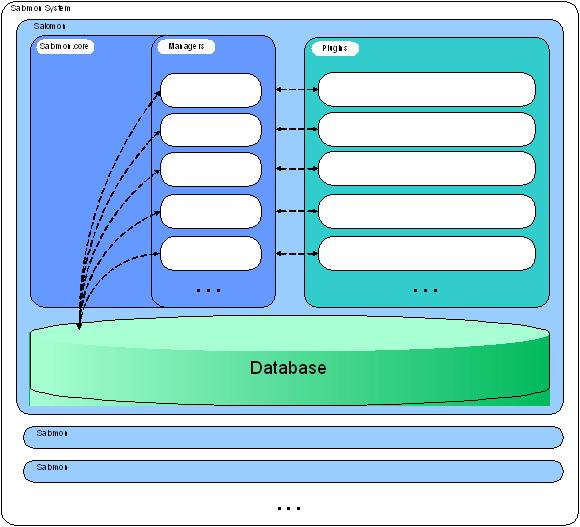
\includegraphics{arch}
	\caption{Architektura systemu}
	\label{fig:arch}
\end{figure}

\pagebreak
Podstawowe za�o�enia projektowe:
\begin{itemize}
    \item ca�a funkcjonalno�� w pluginach. J�dro systemu ma by� jak najmniejsze.
    Jego zadaniem jest stworzenie �rodowiska do realizacji logiki dostarczanej we wtyczkach
    \item otwarta~architektura. Wprowadzenie warstwy po�redniej pomi�dzy baz� danych~a wtyczkami.
    Jej zadaniem jest ukrycie sposobu organizacji danych przez
    wtyczkami. Otwarto��~architektury polega na mo�liwo�ci rozszerzenia tej warstwy
    \item niezale�no�� od platformy. System ma by� niezale�ny od platformy, mo�liwie �atwo przenaszalny.
    Poszczeg�lne cz�ci systemu mog� by� uruchamiane na r�nych
    platformach.
    \item �atwa~adaptacja funkcjonalno�ci zawartej w \emph{Vinlenie}.
    Projekt powsta� jako platforma uruchomieniowa dla logiki zaimplementowanej w programie \emph{Vinlen},
    stworzonego pod kierownictwem prof. Ryszarda Michalskiego.
\end{itemize}


Salomon ma na celu wyeliminowanie ogranicze� oryginalnego
\emph{Vinlena} poprzez wprowadzenie:

\begin{itemize}
    \item kolejkowania zada�
    \item rozproszenia
    \item r�wnoleg�o�ci
    \item rozszerzalno�ci (mechanizm wtyczek)
    \item przeno�no�ci (\emph{Java},\emph{Firebird})
\end{itemize}

\section{Architektura}

%diagram

System zosta� podzielony na 3 g��wne cz�ci: platform�, kontrolery
i~pluginy.

\subsection{Platforma}

Dostarcza podstawowej funkcjonalno�ci  umo�liwiaj�cej prac� ca�ego
systemu,  �aduje odpowiedni kontroler, wczytuje pluginy, uruchamia
zadania. Za poszczeg�lne zadania odpowiadaj� odpowiednie managery.
\\
Managery nie s� dost�pne bezpo�rednio z platformy, ale
przekazywane s� pluginom poprzez klas� \emph{DataEngine}. Dotyczy
to tylko klasy \emph{DataSetManager} i \emph{RuleSetManager},
pozosta�e nie s� dost�pne dla plugin�w. Plugin, zale�nie od
potrzeb, pobiera sobie z niego potrzebny mu manager i za jego
po�rednictwem wykonuje operacje na bazie danych.

\subsubsection{IManagerEngine}
Klasa zarz�dza pozosta�ymi managerami. Utrzymuje jedn� instancj� ka�dego z nich 
i udost�pnia je pozosta�ym klasom z platformy.

\subsubsection{DBManager}
Odpowiada za po��czenie z baz� danych. Dostarcza metod
zapewniaj�cych dost�p do danych przechowywanych w bazie. Swoj�
funkcjonalno�� udost�pnia odpowiednim managerom.

\subsubsection{DataSetManager}
Zarz�dza zbiorami danych. Pozwala tworzy� nowe podzbiory danych na
podstawie zawartych w bazie informacji oraz umo�liwia operowanie
na nich.

\subsubsection{RuleSetManager}
Zarz�dza regu�ami. Pozwala tworzy� nowe regu�y oraz
zarz�dza dost�pem do ju� istniej�cych.

\subsubsection{ProjectManager}
Zarz�dza projektami. Pozwala na utworzenie nowego
projektu, zapisanie bie��cego do bazy danych lub za�adowanie ju�
istniej�cego.

\subsection{Kontrolery}
Kontrolery odpowiadaj� za interakcj�
systemu z otoczeniem. W zale�no�ci od konfiguracji systemu przy
starcie uruchamiany jest jeden z kontroler�w. Kontrolery operuj�
na danych poprzez wsp�lny interfejs, a co za tym idzie: dane
utworzone poprzez jeden z nich s� dost�pne pomi�dzy kolejnymi
uruchomieniami programu dla pozosta�ych kontroler�w.

\subsubsection{LocalController}
 Jest najprostszym kontrolerem. Jego zadaniem jest
zarz�dzanie zadaniami wykonywanymi na lokalnym komputerze. S� one
wykonywane sekwencyjnie. Jego zadaniem jest dostarczenie
interfejsu u�ytkownika pozwalaj�cego na zarz�dzanie projektami,
pluginami i zadaniami.

\subsubsection{ServerController}
Zadaniem tego kontrolera jest dostarczenie interfejsu do
zarz�dzania zdalnymi kontrolerami (\emph{ClientController}). Po
uruchomieniu nas�uchuje na po��czenia od klient�w, rozdziela
zadania oraz wy�wietla ich wyniki.

\subsubsection{ClientController}
Zadaniem tego kontrolera jest odszukanie g��wnego kontrolera
(\emph{ServerController}), zarejestrowanie si� i udost�pnienia mu
swoich us�ug. Ta wersja kontrolera nie posiada GUI, zarz�dzanie
nim odbywa si� za pomoc� klasy \emph{ServerController}.


\subsection{Pluginy}
G��wna funkcjonalno�� zosta�a  przeniesiona
do plugin�w, zadaniem systemu jest tylko zarz�dzanie ich
wykonaniem. Dzi�ki takiemu podej�ciu system jest �atwo skalowalny
i rozszerzalny o nowe mo�liwo�ci. Ka�dy z plugin�w musi
implementowa� nast�puj�ce interfejsy:


\subsubsection{IGraphicPlugin}
Pozwala pobra� parametry od u�ytkownika, kt�re nast�pnie zostan�
przekazane do plugin�w  przed ich wykonaniem. Zawiera dwie metody:
\emph{getSettingsPanel()}  i \emph{getResultPanel()}.  Pierwsza z
metod zwraca panel s�u��cy do konfiguracji pluginu, druga � panel
na kt�rym prezentowane s� wyniki jego dzia�ania.

\subsubsection{IDataPlugin}

Posiada tylko jedn� metod� \emph{doJob()}. Przyjmuje ona jako
parametry obiekt klasy \emph{Environment}, reprezentuj�cy aktualny
stan systemu, \emph{DataEngine}, kt�ry umo�liwia operowanie na
bazie danych i \emph{ISettings}, reprezentuj�cy ustawienia
pluginu. Zwracany jest obiekt klasy \emph{IResult}, stanowi�cy
rezultat wykonania zadania.
\section{Interfejsy plugin�w}

System, dzi�ki swej elastycznej architekturze, pozwala u�ytkownikowi na rozszerzanie jego mo�liwo�ci poprzez definiowanie przez niego w�asnych plugin�w. 
Ca�a funkcjonalno�� zwi�zana z przetwarzaniem plugin�w, konfigurowaniem ich, prezentacj� wynik�w ich dzia�ania oraz komunikacj� przez sie� ukryta jest przed tw�rc� pluginu i nie musi by� brana pod uwag� przy jego projektowaniu i implementacji. Jedyne co musi on zrobi� to zaimplementowa� opisane wy�ej interfejsy.
By system m�g� skorzysta� z nowych plugin�w nale�y doda� do tabeli plugins odpowiedni wpis, umo�liwiaj�cy systemowi zlokalizowanie i �ci�gni�cie pluginu. 
Obecna wersja systemu obs�uguje tylko pluginy w postaci archiw�w jar.

Ka�dy plugin by m�g� by� przetwarzany przez system musi
implementowa� nast�puj�ce interfejsy:

\subsection{IPlugin}

    \paragraph{getDescription()} - zwraca obiekt klasy
    \emph{Description} zawieraj�cy opis pluginu (nazw�, lokalizacj�,
    wersj� itp.)

\subsection{IDataPlugin}
    \paragraph{doJob()} - metoda wykonuje g��wne zadanie pluginu

\subsection{IGraphicPlugin}

    \paragraph{getSettingComponent()} - zwraca obiekt
    implementuj�cy interfejs \emph{ISettingComponent}

    \paragraph{getResultComponent()} - zwraca obiekt implementuj�cy
    interfejs \emph{IResultComponent}\\



Interfejs \emph{IGraphicComponent} zapewnia interakcj� z
u�ytkownikiem. Jego metody zwracaj� komponenty pozwalaj�ce na
modyfikacj� ustawie� pluginu oraz na wy�wietlenie rezultatu jego
dzia�ania. Obiekty zwracane przez metody tego interfejsu
implementuj� interfejsy:

\subsection{ISettingComponent}

    \paragraph{getComponent(ISettings settings)} - zwraca graficzny
    komponent s�u��cy do edycji ustawie� pluginu. Jest on wype�niany
    warto�ciami przekazanymi w obiekcie \emph{ISettings}.

    \paragraph{getSettings()} - zwraca ustawienia pluginu

    \paragraph{getDefaultSettings()} - zwraca domy�lne ustawienia
    pluginu. Wykorzystywana gdy u�ytkownik nie wprowadzi� w�asnych
    ustawie�

\subsection{IResultComponent}

    \paragraph{getComponent(IResult result)} - zwraca graficzny
    komponent wy�wietlaj�cy rezultat wykonania pluginu. Wype�niany
    jest on na podstawie obiektu  \emph{IResult} zwr�conego wcze�niej
    przez metod� \emph{doJob()}.

    \paragraph{getDefaultResult()} - zwraca domy�lny rezultat wykonania pluginu

\subsection{ISettings}Implementowany przez obiekt reprezentuj�cy
ustawienia pluginu.

    \paragraph{parseSettings(String settings)} - metoda inicjalizuje obiekt klasy
    \emph{ISettings}  na podstawie jego  tekstowej reprezentacji.
    U�ywana przy �adowaniu ustawie� pluginu z  bazy danych

    \paragraph{settingsToString()} - zwraca tekstow� reprezentacj�
    obiektu klasy \emph{ISettings}. U�ywana przy zapisie ustawie� pluginu do
    bazy danych

\subsection{IResult} Implementowany przez obiekt reprezentuj�cy rezultat
dzia�ania pluginu.

    \paragraph{parseResult(String result)}- metoda inicjalizuje obiekt klasy
    \emph{IResult}  na podstawie jego  tekstowej reprezentacji.
    U�ywana przy �adowaniu rezultatu dzia�ania pluginu z bazy danych

    \paragraph{resultToString()} - zwraca tekstow� reprezentacj� obiektu klasy
    \emph{IResult}. U�ywana przy zapisie rezultatu dzia�ania pluginu do bazy danych

\section{Opis bazy danych}sz

Do przechowywania danych wykorzystywanych przez system
wykorzystana zosta�a baza danych. Dane zosta�y zorganizowane w
nast�puj�cych tabelach:

\paragraph{Projects}

Tabela zawiera nag��wki projekt�w, do kt�rych odnosz� si� rekordy
z tabeli Tasks.

\begin{itemize}
    \item \emph{project\_id} - identyfikator projektu
    \item \emph{name} - nazwa
    \item \emph{info} - dodatkowy opis
\end{itemize}

\paragraph{Plugins}
Tabela zawiera informacje o pluginach, kt�re mog� by� wykorzystane
przez system. Przechowuje dane o ich nazwach i lokalizacjach, sk�d
mog� by� pobrane.
\begin{itemize}
    \item \emph{plugin\_id} - identyfikator pluginu
    \item \emph{name} - nazwa
    \item \emph{info} - dodatkowy opis
    \item \emph{location} - lokalizacja pluginu.
\end{itemize}

\paragraph{Tasks}
 Tabela zawiera zapis wykonania poszczeg�lnych task�w . Dla ka�dego
zadania przechowywane s� dane o pluginie, kt�ry zosta�
wykorzystany do wykonania zadania, projekcie, w ramach kt�rego
zadanie zosta�o zapisane, ustawienia, z jakimi zosta�o wykonane,
rezultat zadania oraz status, w jakim pozostaje po wykonaniu.

\begin{itemize}
    \item \emph{task\_id} - identyfikator taska
    \item \emph{project\_id} - identyfikator projektu, do kt�rego nale�y task
    \item \emph{plugin\_id} - identyfikator pluginu, kt�ry wykonywany jest w ramach tego taska
    \item \emph{name} - nazwa
    \item \emph{info} - dodatkowy opis
    \item \emph{plugin\_settings} - ustawienia pocz�tkowe pluginu
    \item \emph{plugin\_result} - rezultat dzia�ania pluginu
    \item \emph{status} - status wykonania taska
\end{itemize}

\paragraph{Datasets}
Zawiera nag��wki zbior�w zada�.
\begin{itemize}
    \item \emph{dataset\_id} - identyfikator zbioru danych
    \item \emph{dataset\_name} - nazwa
    \item \emph{info} - dodatkowy opis
\end{itemize}

\paragraph{Dataset\_items}
Zawiera definicje zbior�w zada�. Zbi�r danych definiowany jest
przez nazw� tabeli oraz warunki, jaki ograniczaj� rekordy w tej
tabeli.
\begin{itemize}
    \item \emph{dataset\_item\_id} - identyfikator elementu zbioru danych
    \item \emph{dataset\_id} - identyfikator zbioru danych do kt�rego nale�y
element
    \item \emph{table\_name} - nazwa tabeli
    \item \emph{condition} - warunek ograniczaj�cy zakres danych
\end{itemize}
    Relacje mi�dzy nimi zobrazowane s� na
poni�szym rysunku:


\end{document}
